\batchmode

\documentclass[12pt,a4paper]{report}
\RequirePackage{ifthen}


\usepackage{german}
\usepackage{graphicx,makeidx,showidx,index}
\newindex{default}{idx}{ind}{Schlagwortverzeichnis}
\usepackage{epsfig}
\usepackage[german]{varioref}
\usepackage[latin1]{inputenc}


\setcounter{tocdepth}{2}
\pagestyle{headings}


\usepackage[dvips]{color}


\pagecolor[gray]{.7}

\usepackage[latin1]{inputenc}



\makeatletter

\makeatletter
\count@=\the\catcode`\_ \catcode`\_=8 
\newenvironment{tex2html_wrap}{}{}%
\catcode`\<=12\catcode`\_=\count@
\newcommand{\providedcommand}[1]{\expandafter\providecommand\csname #1\endcsname}%
\newcommand{\renewedcommand}[1]{\expandafter\providecommand\csname #1\endcsname{}%
  \expandafter\renewcommand\csname #1\endcsname}%
\newcommand{\newedenvironment}[1]{\newenvironment{#1}{}{}\renewenvironment{#1}}%
\let\newedcommand\renewedcommand
\let\renewedenvironment\newedenvironment
\makeatother
\let\mathon=$
\let\mathoff=$
\ifx\AtBeginDocument\undefined \newcommand{\AtBeginDocument}[1]{}\fi
\newbox\sizebox
\setlength{\hoffset}{0pt}\setlength{\voffset}{0pt}
\addtolength{\textheight}{\footskip}\setlength{\footskip}{0pt}
\addtolength{\textheight}{\topmargin}\setlength{\topmargin}{0pt}
\addtolength{\textheight}{\headheight}\setlength{\headheight}{0pt}
\addtolength{\textheight}{\headsep}\setlength{\headsep}{0pt}
\setlength{\textwidth}{349pt}
\newwrite\lthtmlwrite
\makeatletter
\let\realnormalsize=\normalsize
\global\topskip=2sp
\def\preveqno{}\let\real@float=\@float \let\realend@float=\end@float
\def\@float{\let\@savefreelist\@freelist\real@float}
\def\liih@math{\ifmmode$\else\bad@math\fi}
\def\end@float{\realend@float\global\let\@freelist\@savefreelist}
\let\real@dbflt=\@dbflt \let\end@dblfloat=\end@float
\let\@largefloatcheck=\relax
\let\if@boxedmulticols=\iftrue
\def\@dbflt{\let\@savefreelist\@freelist\real@dbflt}
\def\adjustnormalsize{\def\normalsize{\mathsurround=0pt \realnormalsize
 \parindent=0pt\abovedisplayskip=0pt\belowdisplayskip=0pt}%
 \def\phantompar{\csname par\endcsname}\normalsize}%
\def\lthtmltypeout#1{{\let\protect\string \immediate\write\lthtmlwrite{#1}}}%
\newcommand\lthtmlhboxmathA{\adjustnormalsize\setbox\sizebox=\hbox\bgroup\kern.05em }%
\newcommand\lthtmlhboxmathB{\adjustnormalsize\setbox\sizebox=\hbox to\hsize\bgroup\hfill }%
\newcommand\lthtmlvboxmathA{\adjustnormalsize\setbox\sizebox=\vbox\bgroup %
 \let\ifinner=\iffalse \let\)\liih@math }%
\newcommand\lthtmlboxmathZ{\@next\next\@currlist{}{\def\next{\voidb@x}}%
 \expandafter\box\next\egroup}%
\newcommand\lthtmlmathtype[1]{\gdef\lthtmlmathenv{#1}}%
\newcommand\lthtmllogmath{\dimen0\ht\sizebox \advance\dimen0\dp\sizebox
  \ifdim\dimen0>.95\vsize
   \lthtmltypeout{%
*** image for \lthtmlmathenv\space is too tall at \the\dimen0, reducing to .95 vsize ***}%
   \ht\sizebox.95\vsize \dp\sizebox\z@ \fi
  \lthtmltypeout{l2hSize %
:\lthtmlmathenv:\the\ht\sizebox::\the\dp\sizebox::\the\wd\sizebox.\preveqno}}%
\newcommand\lthtmlfigureA[1]{\let\@savefreelist\@freelist
       \lthtmlmathtype{#1}\lthtmlvboxmathA}%
\newcommand\lthtmlpictureA{\bgroup\catcode`\_=8 \lthtmlpictureB}%
\newcommand\lthtmlpictureB[1]{\lthtmlmathtype{#1}\egroup
       \let\@savefreelist\@freelist \lthtmlhboxmathB}%
\newcommand\lthtmlpictureZ[1]{\hfill\lthtmlfigureZ}%
\newcommand\lthtmlfigureZ{\lthtmlboxmathZ\lthtmllogmath\copy\sizebox
       \global\let\@freelist\@savefreelist}%
\newcommand\lthtmldisplayA{\bgroup\catcode`\_=8 \lthtmldisplayAi}%
\newcommand\lthtmldisplayAi[1]{\lthtmlmathtype{#1}\egroup\lthtmlvboxmathA}%
\newcommand\lthtmldisplayB[1]{\edef\preveqno{(\theequation)}%
  \lthtmldisplayA{#1}\let\@eqnnum\relax}%
\newcommand\lthtmldisplayZ{\lthtmlboxmathZ\lthtmllogmath\lthtmlsetmath}%
\newcommand\lthtmlinlinemathA{\bgroup\catcode`\_=8 \lthtmlinlinemathB}
\newcommand\lthtmlinlinemathB[1]{\lthtmlmathtype{#1}\egroup\lthtmlhboxmathA
  \vrule height1.5ex width0pt }%
\newcommand\lthtmlinlineA{\bgroup\catcode`\_=8 \lthtmlinlineB}%
\newcommand\lthtmlinlineB[1]{\lthtmlmathtype{#1}\egroup\lthtmlhboxmathA}%
\newcommand\lthtmlinlineZ{\egroup\expandafter\ifdim\dp\sizebox>0pt %
  \expandafter\centerinlinemath\fi\lthtmllogmath\lthtmlsetinline}
\newcommand\lthtmlinlinemathZ{\egroup\expandafter\ifdim\dp\sizebox>0pt %
  \expandafter\centerinlinemath\fi\lthtmllogmath\lthtmlsetmath}
\newcommand\lthtmlindisplaymathZ{\egroup %
  \centerinlinemath\lthtmllogmath\lthtmlsetmath}
\def\lthtmlsetinline{\hbox{\vrule width.1em \vtop{\vbox{%
  \kern.1em\copy\sizebox}\ifdim\dp\sizebox>0pt\kern.1em\else\kern.3pt\fi
  \ifdim\hsize>\wd\sizebox \hrule depth1pt\fi}}}
\def\lthtmlsetmath{\hbox{\vrule width.1em\kern-.05em\vtop{\vbox{%
  \kern.1em\kern0.8 pt\hbox{\hglue.17em\copy\sizebox\hglue0.8 pt}}\kern.3pt%
  \ifdim\dp\sizebox>0pt\kern.1em\fi \kern0.8 pt%
  \ifdim\hsize>\wd\sizebox \hrule depth1pt\fi}}}
\def\centerinlinemath{%
  \dimen1=\ifdim\ht\sizebox<\dp\sizebox \dp\sizebox\else\ht\sizebox\fi
  \advance\dimen1by.5pt \vrule width0pt height\dimen1 depth\dimen1 
 \dp\sizebox=\dimen1\ht\sizebox=\dimen1\relax}

\def\lthtmlcheckvsize{\ifdim\ht\sizebox<\vsize 
  \ifdim\wd\sizebox<\hsize\expandafter\hfill\fi \expandafter\vfill
  \else\expandafter\vss\fi}%
\providecommand{\selectlanguage}[1]{}%
\makeatletter \tracingstats = 1 


\begin{document}
\pagestyle{empty}\thispagestyle{empty}\lthtmltypeout{}%
\lthtmltypeout{latex2htmlLength hsize=\the\hsize}\lthtmltypeout{}%
\lthtmltypeout{latex2htmlLength vsize=\the\vsize}\lthtmltypeout{}%
\lthtmltypeout{latex2htmlLength hoffset=\the\hoffset}\lthtmltypeout{}%
\lthtmltypeout{latex2htmlLength voffset=\the\voffset}\lthtmltypeout{}%
\lthtmltypeout{latex2htmlLength topmargin=\the\topmargin}\lthtmltypeout{}%
\lthtmltypeout{latex2htmlLength topskip=\the\topskip}\lthtmltypeout{}%
\lthtmltypeout{latex2htmlLength headheight=\the\headheight}\lthtmltypeout{}%
\lthtmltypeout{latex2htmlLength headsep=\the\headsep}\lthtmltypeout{}%
\lthtmltypeout{latex2htmlLength parskip=\the\parskip}\lthtmltypeout{}%
\lthtmltypeout{latex2htmlLength oddsidemargin=\the\oddsidemargin}\lthtmltypeout{}%
\makeatletter
\if@twoside\lthtmltypeout{latex2htmlLength evensidemargin=\the\evensidemargin}%
\else\lthtmltypeout{latex2htmlLength evensidemargin=\the\oddsidemargin}\fi%
\lthtmltypeout{}%
\makeatother
\setcounter{page}{1}
\onecolumn

% !!! IMAGES START HERE !!!

\setcounter{tocdepth}{2}
{\newpage\clearpage
\lthtmlfigureA{parbox19}%
\begin{parbox}[b][17cm][s]{15cm}
\par
\textbf{Copyright \copyright 2005-2006 Jan Kechel, Martin Klink, Jonas Heese, Andreas Bachmann}
\par
Permission is granted to copy, distribute and/or modify this document
under the terms of the GNU Free Documentation License, Version 1.2
or any later version published by the Free Software Foundation;
with no Invariant Sections, no Front-Cover Texts, and no Back-Cover
Texts.  A copy of the license is included in the section entitled ''GNU
Free Documentation License''.
\end{parbox}%
\lthtmlfigureZ
\lthtmlcheckvsize\clearpage}

\stepcounter{chapter}
\stepcounter{section}
\stepcounter{section}
{\newpage\clearpage
\lthtmlfigureA{figure48}%
\begin{figure}
\epsfig{file=logo_teamfound}

\end{figure}%
\lthtmlfigureZ
\lthtmlcheckvsize\clearpage}

\stepcounter{subsection}
{\newpage\clearpage
\lthtmlfigureA{figure58}%
\begin{figure}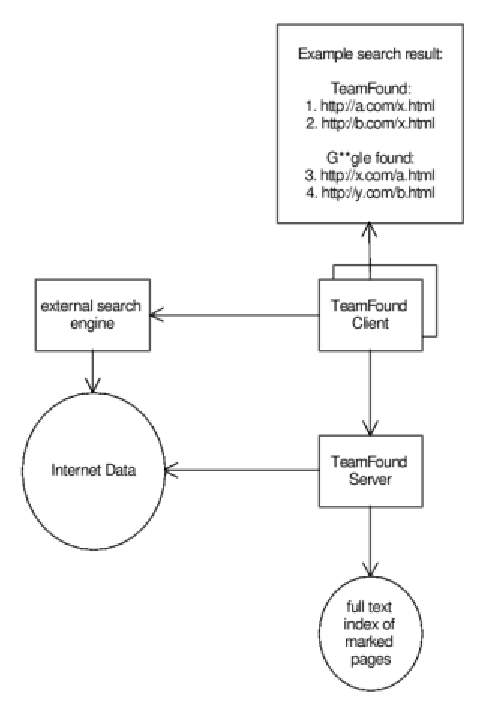
\epsfig{file=architecture1}

\end{figure}%
\lthtmlfigureZ
\lthtmlcheckvsize\clearpage}

\stepcounter{subsection}
\stepcounter{subsubsection}
\stepcounter{subsubsection}
\stepcounter{chapter}
\stepcounter{section}
\stepcounter{subsection}
\stepcounter{subsection}
\stepcounter{section}
\stepcounter{subsection}
\stepcounter{subsubsection}
{\newpage\clearpage
\lthtmlinlinemathA{tex2html_wrap_inline690}%
$Analyzer$%
\lthtmlinlinemathZ
\lthtmlcheckvsize\clearpage}

{\newpage\clearpage
\lthtmlinlinemathA{tex2html_wrap_inline692}%
$Felder$%
\lthtmlinlinemathZ
\lthtmlcheckvsize\clearpage}

\stepcounter{subsubsection}
\stepcounter{paragraph}
\stepcounter{paragraph}
{\newpage\clearpage
\lthtmlinlinemathA{tex2html_wrap_inline694}%
$Whitespaces$%
\lthtmlinlinemathZ
\lthtmlcheckvsize\clearpage}

\stepcounter{paragraph}
\stepcounter{subsection}
\stepcounter{subsection}
\stepcounter{section}
{\newpage\clearpage
\lthtmlpictureA{tex2html_wrap5266}%
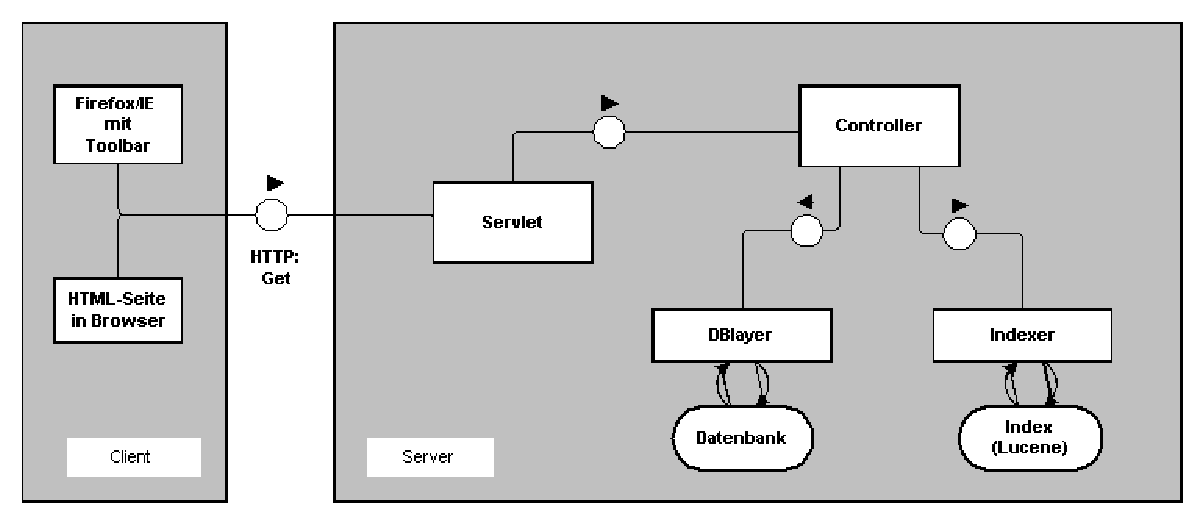
\includegraphics[width=16cm]{bilder/aufbau2.eps}%
\lthtmlpictureZ
\lthtmlcheckvsize\clearpage}

\stepcounter{subsection}
\stepcounter{subsection}
\stepcounter{subsection}
\stepcounter{subsection}
\stepcounter{section}
\stepcounter{subsection}
{\newpage\clearpage
\lthtmlpictureA{tex2html_wrap5287}%
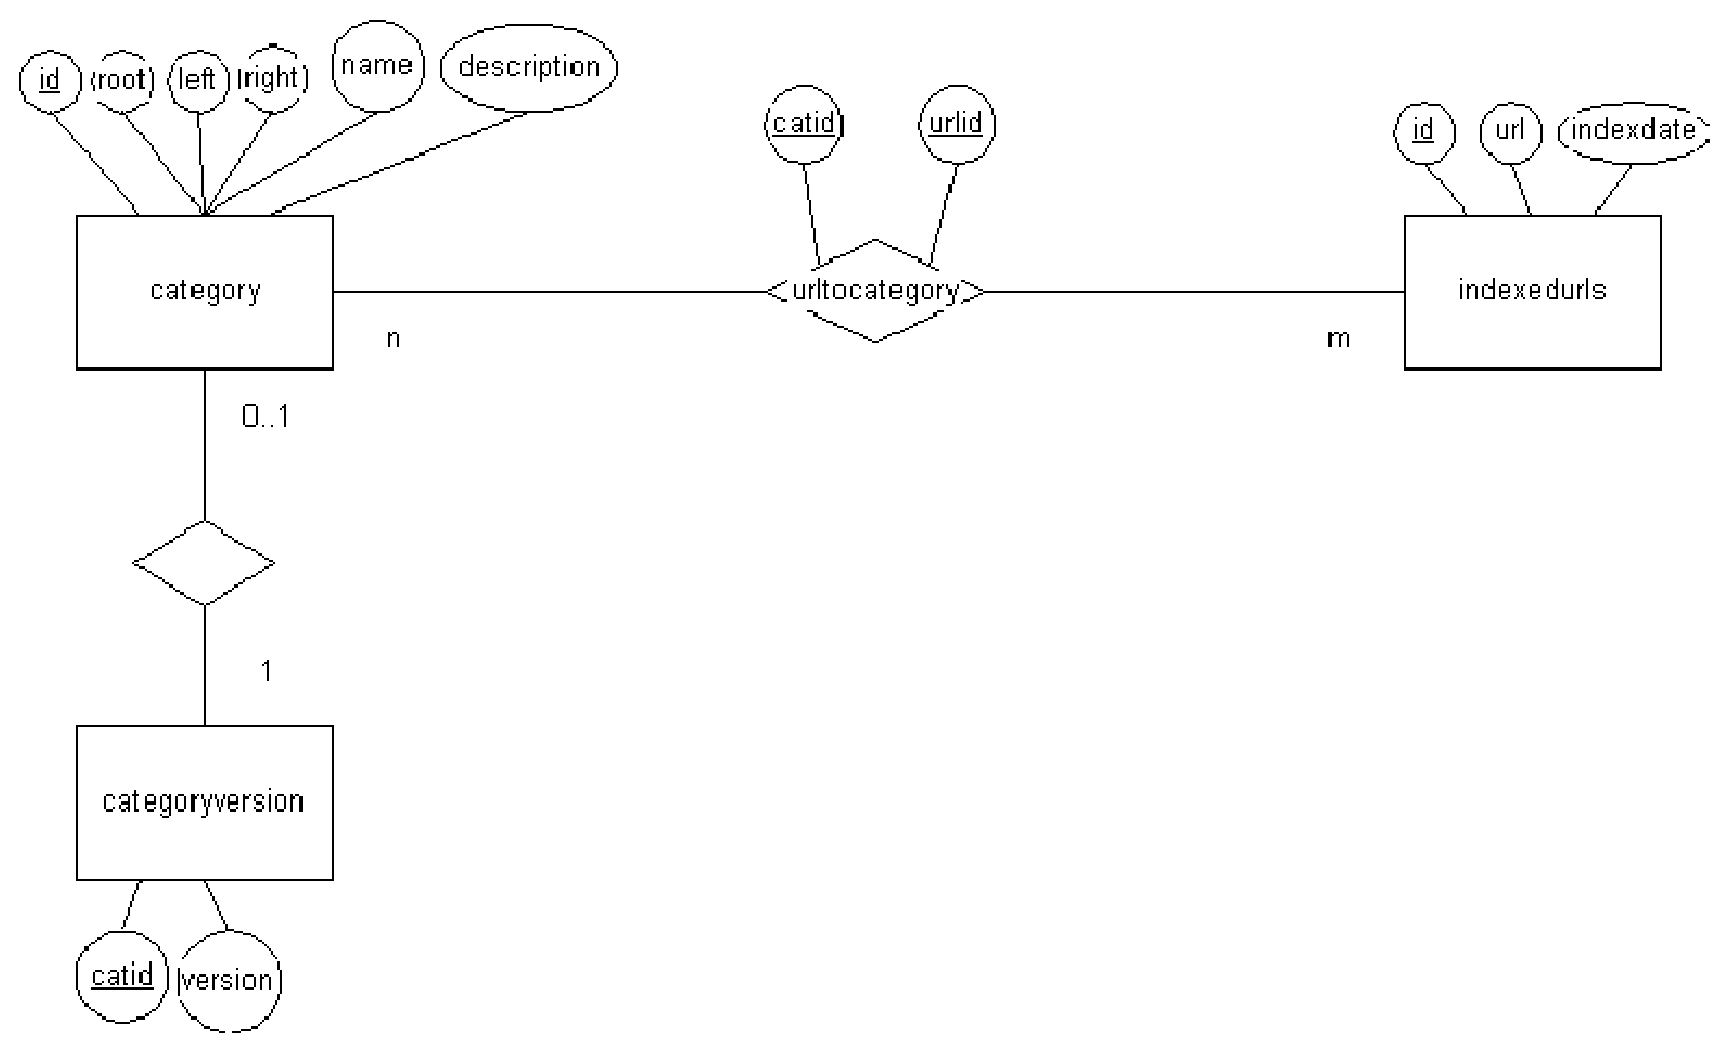
\includegraphics[width=16cm]{bilder/db.eps}%
\lthtmlpictureZ
\lthtmlcheckvsize\clearpage}

{\newpage\clearpage
\lthtmlinlinemathA{tex2html_wrap_inline696}%
$category$%
\lthtmlinlinemathZ
\lthtmlcheckvsize\clearpage}

{\newpage\clearpage
\lthtmlinlinemathA{tex2html_wrap_inline698}%
$categoryversion$%
\lthtmlinlinemathZ
\lthtmlcheckvsize\clearpage}

{\newpage\clearpage
\lthtmlinlinemathA{tex2html_wrap_inline700}%
$indexedurl$%
\lthtmlinlinemathZ
\lthtmlcheckvsize\clearpage}

\stepcounter{subsection}
{\newpage\clearpage
\lthtmlinlinemathA{tex2html_wrap_inline704}%
$Analyser$%
\lthtmlinlinemathZ
\lthtmlcheckvsize\clearpage}

\stepcounter{subsection}
{\newpage\clearpage
\lthtmlpictureA{tex2html_wrap5299}%
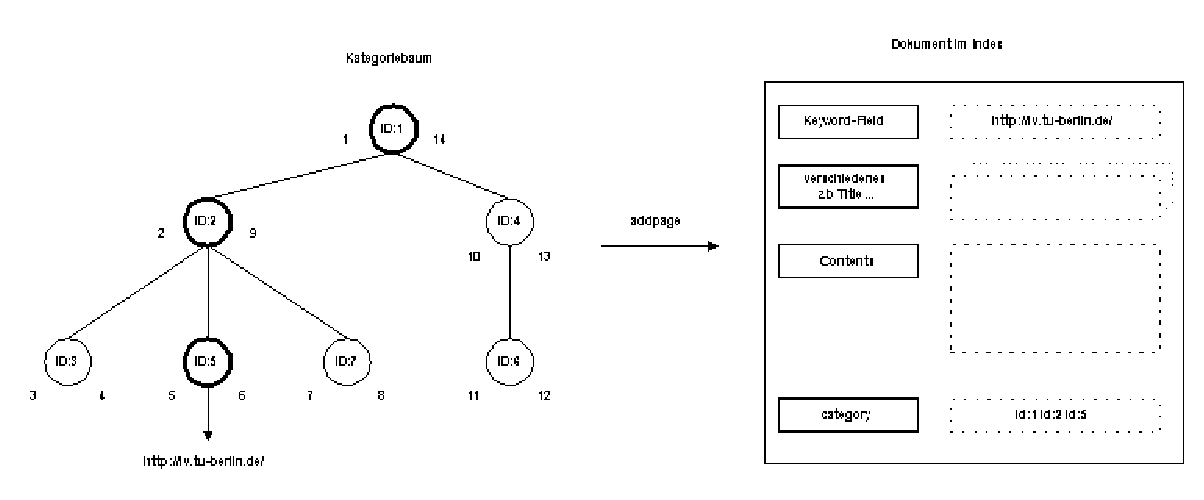
\includegraphics[width=16cm]{bilder/katstruktur.eps}%
\lthtmlpictureZ
\lthtmlcheckvsize\clearpage}

\stepcounter{section}
\stepcounter{subsection}
{\newpage\clearpage
\lthtmlpictureA{tex2html_wrap5305}%
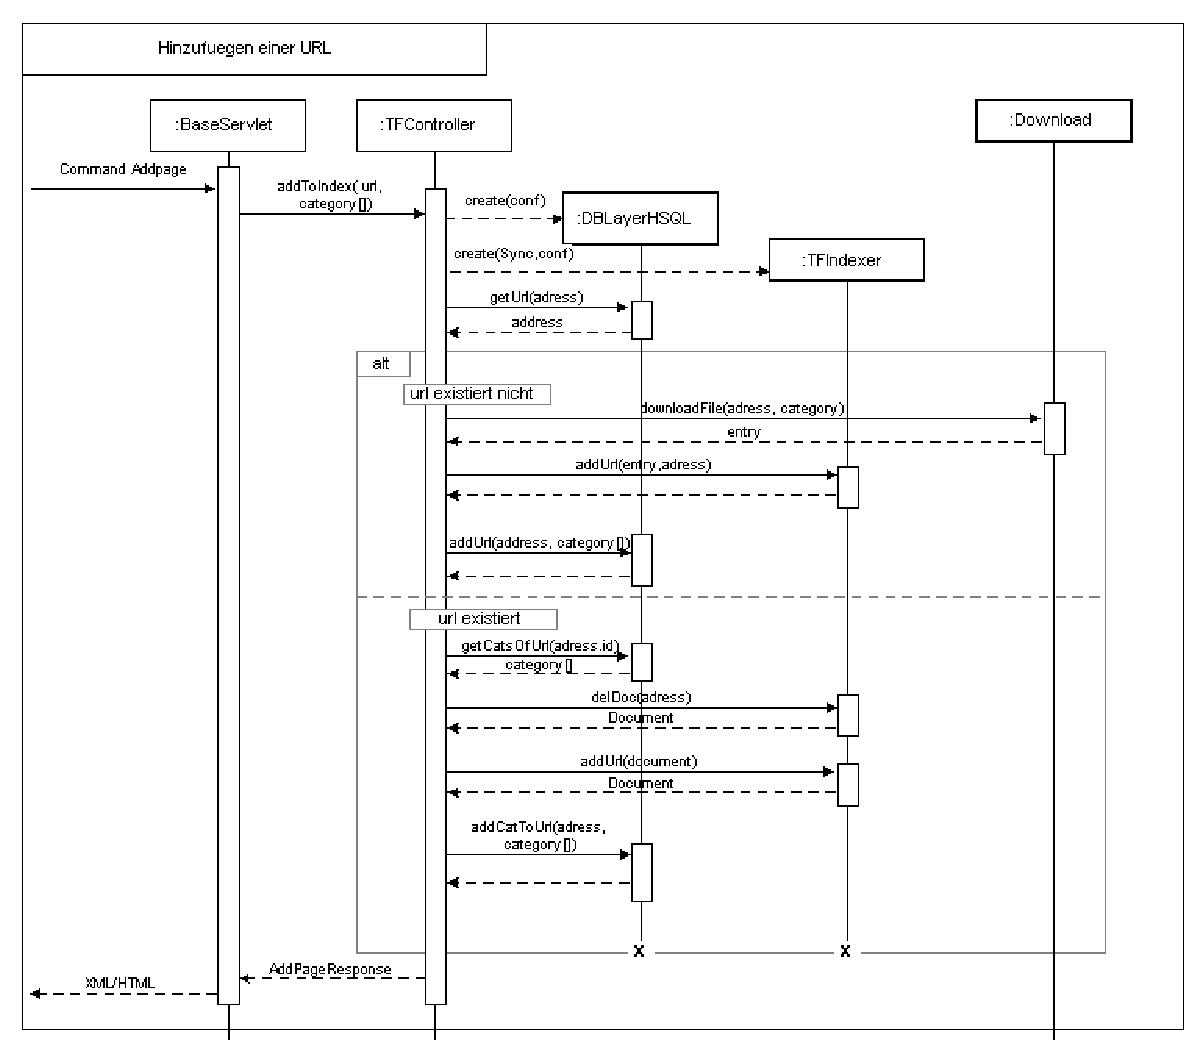
\includegraphics[width=16cm]{bilder/ablaufaddpage1.eps}%
\lthtmlpictureZ
\lthtmlcheckvsize\clearpage}

{\newpage\clearpage
\lthtmlinlinemathA{tex2html_wrap_inline708}%
$Get$%
\lthtmlinlinemathZ
\lthtmlcheckvsize\clearpage}

\stepcounter{subsection}
{\newpage\clearpage
\lthtmlpictureA{tex2html_wrap5311}%
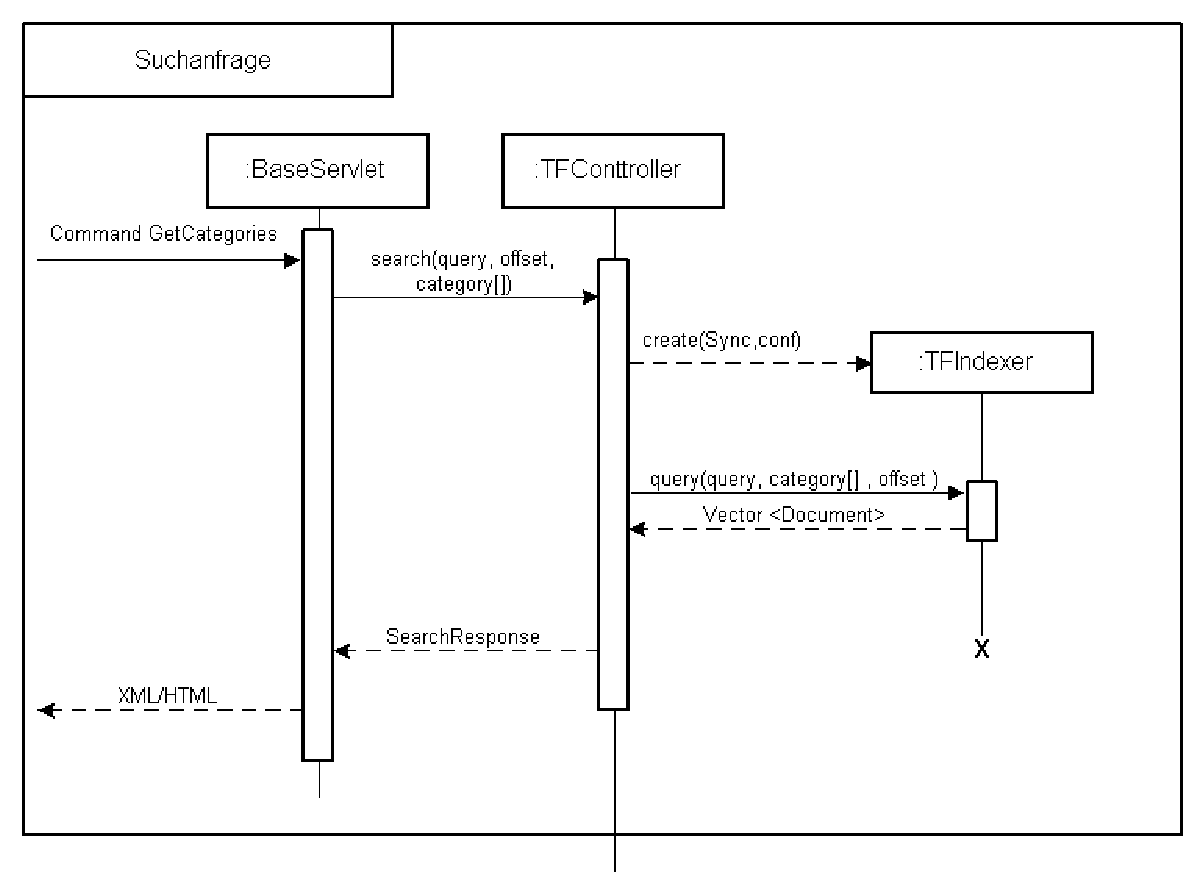
\includegraphics[width=14cm]{bilder/search.eps}%
\lthtmlpictureZ
\lthtmlcheckvsize\clearpage}

{\newpage\clearpage
\lthtmlinlinemathA{tex2html_wrap_inline710}%
$QuerySyntax$%
\lthtmlinlinemathZ
\lthtmlcheckvsize\clearpage}

{\newpage\clearpage
\lthtmlinlinemathA{tex2html_wrap_inline712}%
$Query$%
\lthtmlinlinemathZ
\lthtmlcheckvsize\clearpage}

{\newpage\clearpage
\lthtmlinlinemathA{tex2html_wrap_inline716}%
$Response$%
\lthtmlinlinemathZ
\lthtmlcheckvsize\clearpage}

\stepcounter{subsection}
{\newpage\clearpage
\lthtmlpictureA{tex2html_wrap5320}%
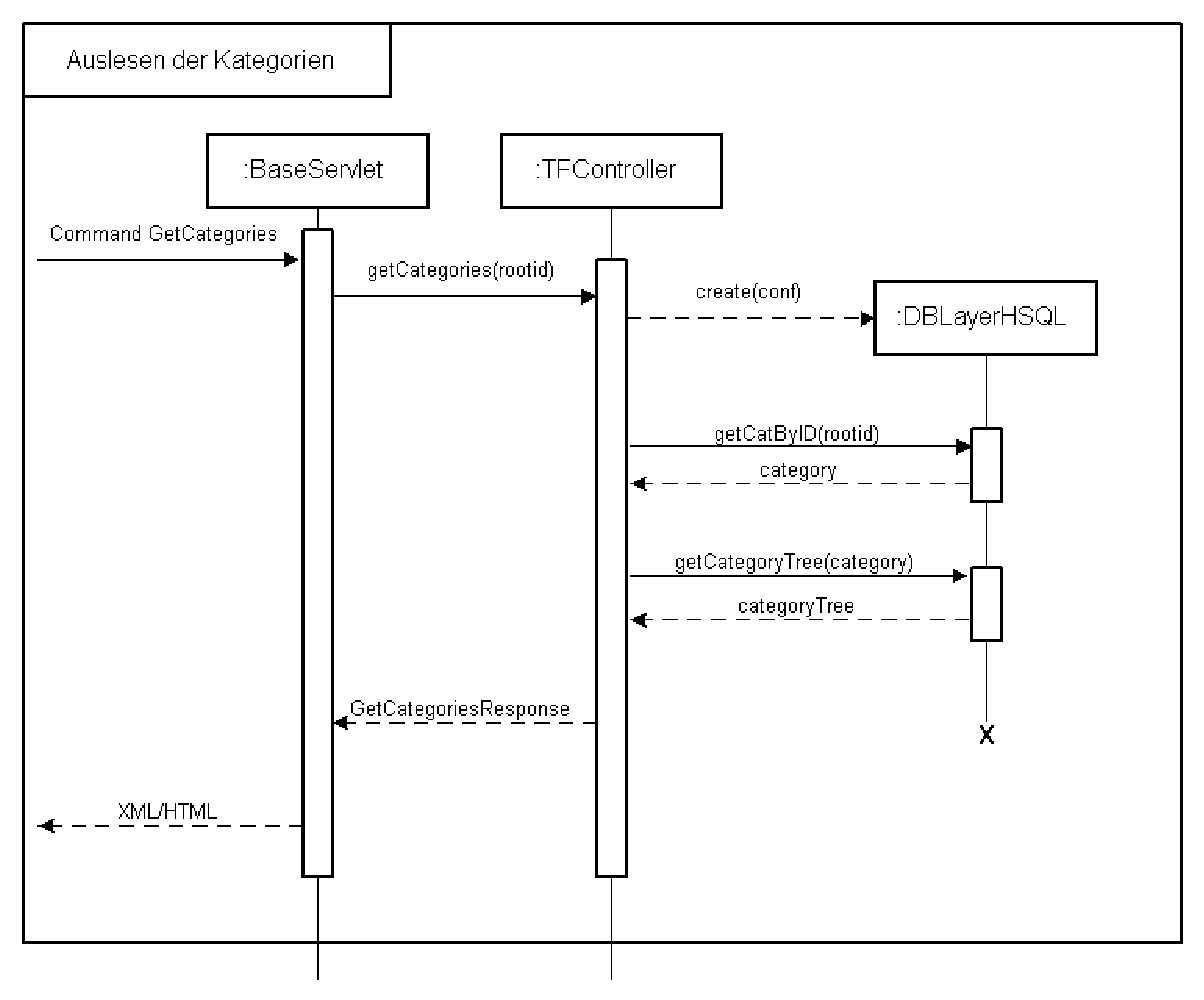
\includegraphics[width=14cm]{bilder/getcat.eps}%
\lthtmlpictureZ
\lthtmlcheckvsize\clearpage}

\stepcounter{section}
\stepcounter{section}
\stepcounter{chapter}
\stepcounter{section}
\stepcounter{section}
\stepcounter{subsection}
\stepcounter{subsection}
\stepcounter{section}
\stepcounter{subsubsection}
\stepcounter{subsubsection}
{\newpage\clearpage
\lthtmlinlinemathA{tex2html_wrap_inline718}%
$<$%
\lthtmlinlinemathZ
\lthtmlcheckvsize\clearpage}

{\newpage\clearpage
\lthtmlinlinemathA{tex2html_wrap_inline720}%
$>$%
\lthtmlinlinemathZ
\lthtmlcheckvsize\clearpage}

\stepcounter{paragraph}
\stepcounter{chapter}
\stepcounter{section}
{\newpage\clearpage
\lthtmlfigureA{figure506}%
\begin{figure}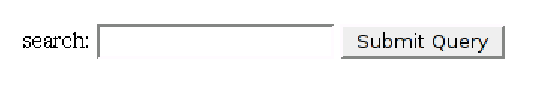
\epsfig{file=webclient}

\end{figure}%
\lthtmlfigureZ
\lthtmlcheckvsize\clearpage}

\stepcounter{subsection}
\stepcounter{section}
{\newpage\clearpage
\lthtmlfigureA{figure537}%
\begin{figure}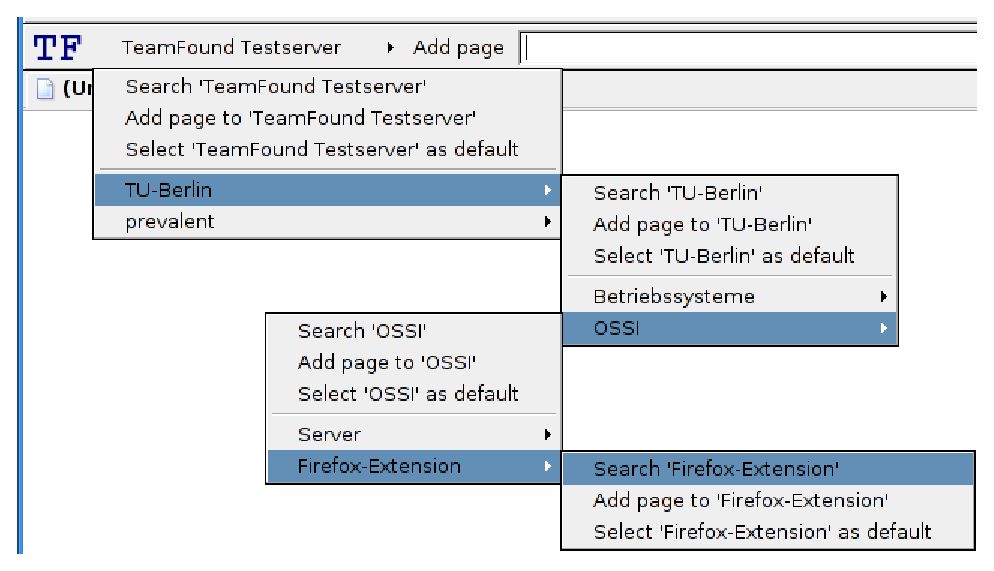
\epsfig{file=ffextension-kategorien}

\end{figure}%
\lthtmlfigureZ
\lthtmlcheckvsize\clearpage}

\stepcounter{subsection}
\stepcounter{subsection}
{\newpage\clearpage
\lthtmlfigureA{figure555}%
\begin{figure}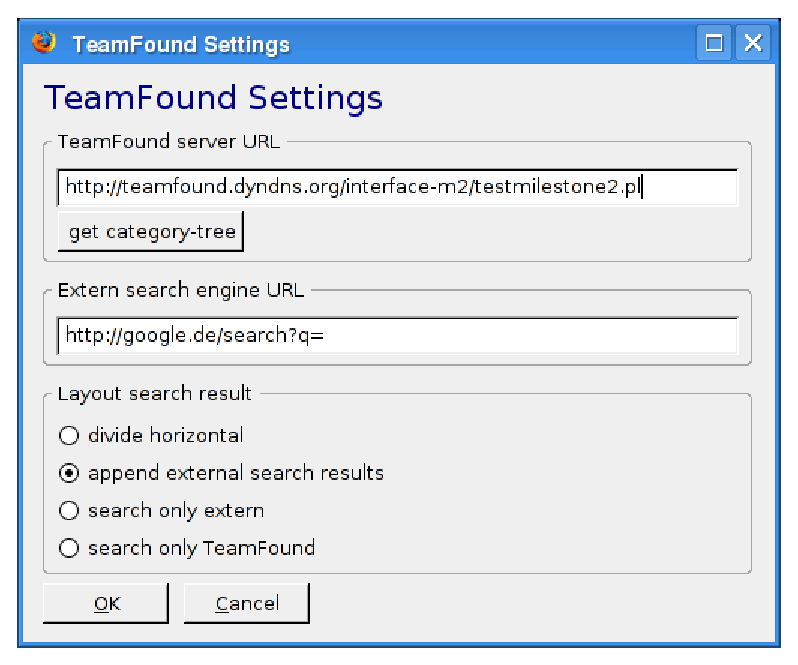
\epsfig{file=ffextension-settings}

\end{figure}%
\lthtmlfigureZ
\lthtmlcheckvsize\clearpage}

{\newpage\clearpage
\lthtmlfigureA{figure560}%
\begin{figure}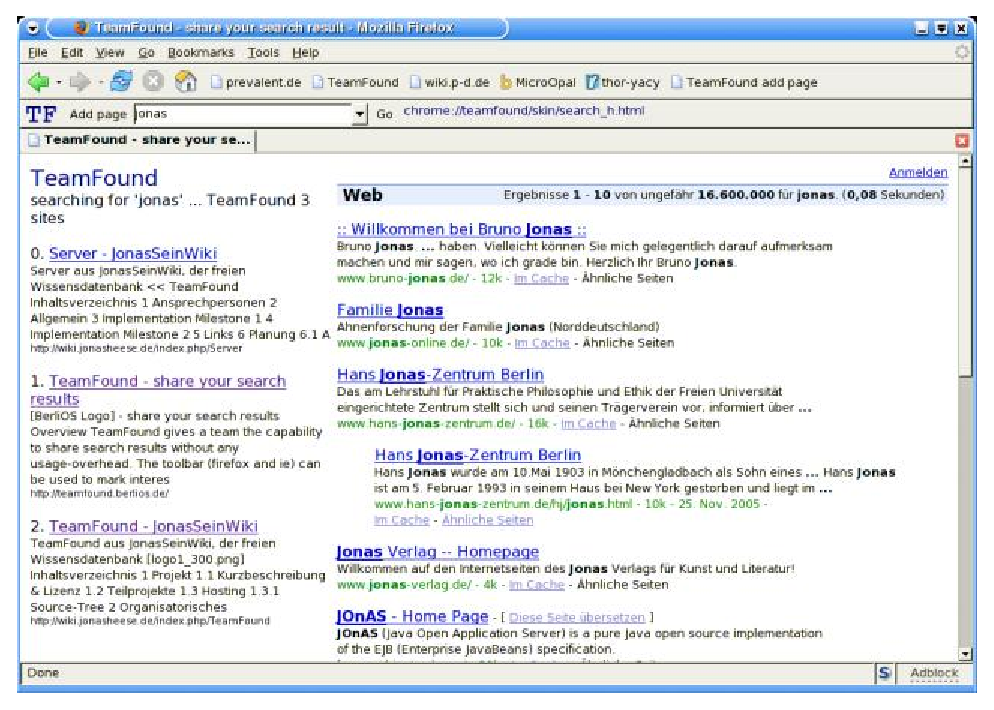
\epsfig{file=screenshot-search-server-0.1-firefox-toolbar-0.4.eps}

\end{figure}%
\lthtmlfigureZ
\lthtmlcheckvsize\clearpage}

\stepcounter{section}
\stepcounter{subsection}
\stepcounter{paragraph}
\stepcounter{paragraph}
\stepcounter{paragraph}
\stepcounter{subsection}
\stepcounter{subsection}
\stepcounter{paragraph}
\stepcounter{paragraph}
\stepcounter{paragraph}
\stepcounter{subsection}
\stepcounter{paragraph}
\stepcounter{paragraph}
\stepcounter{paragraph}
\stepcounter{paragraph}
\stepcounter{paragraph}
\stepcounter{subsection}
\stepcounter{subsection}
\stepcounter{subsection}
\stepcounter{subsection}
\stepcounter{paragraph}
\stepcounter{paragraph}
{\newpage\clearpage
\lthtmlfigureA{figure674}%
\begin{figure}\begin{center}
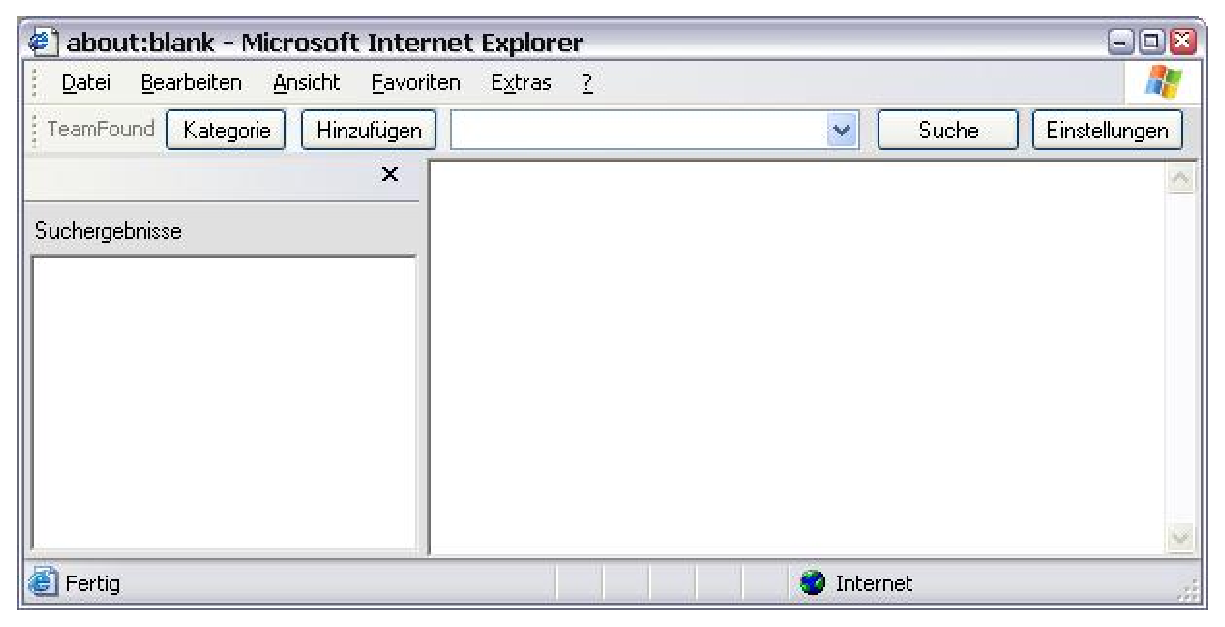
\epsfig{file=bilder/ietoolbar, width=12cm}
\end{center}

\end{figure}%
\lthtmlfigureZ
\lthtmlcheckvsize\clearpage}

\stepcounter{paragraph}
\stepcounter{paragraph}
\stepcounter{subsection}
\stepcounter{chapter}
\stepcounter{section}
\stepcounter{section}
\stepcounter{section}
\stepcounter{section}
\stepcounter{subsection}
\stepcounter{subsection}
\stepcounter{subsection}
\stepcounter{subsection}
\stepcounter{chapter}
\stepcounter{chapter}
\stepcounter{section}
\stepcounter{subsection}
\stepcounter{subsubsection}
\stepcounter{subsubsection}
\stepcounter{subsubsection}
\stepcounter{subsubsection}
\stepcounter{paragraph}
\stepcounter{subsection}
\stepcounter{subsubsection}
\stepcounter{subsubsection}
\stepcounter{subsubsection}
\stepcounter{subsection}
\stepcounter{subsubsection}
\stepcounter{subsubsection}
\stepcounter{subsubsection}
\stepcounter{subsection}
\stepcounter{subsubsection}
\stepcounter{subsubsection}
\stepcounter{subsubsection}
\stepcounter{subsection}
\stepcounter{subsubsection}
\stepcounter{subsubsection}
\stepcounter{subsubsection}
\stepcounter{subsection}
\stepcounter{subsubsection}
\stepcounter{subsubsection}
\stepcounter{subsubsection}
\stepcounter{subsection}
\stepcounter{chapter}
\stepcounter{section}
\stepcounter{subsection}
\stepcounter{subsubsection}
\stepcounter{paragraph}
\stepcounter{paragraph}
\stepcounter{paragraph}
\stepcounter{paragraph}
\stepcounter{paragraph}
\stepcounter{paragraph}
\stepcounter{paragraph}
\stepcounter{paragraph}
\stepcounter{subsubsection}
\stepcounter{paragraph}
\stepcounter{paragraph}
\stepcounter{subsubsection}
\stepcounter{paragraph}
\stepcounter{paragraph}
\stepcounter{subsection}
\stepcounter{subsubsection}
\stepcounter{paragraph}
\stepcounter{paragraph}
\stepcounter{paragraph}
\stepcounter{paragraph}
\stepcounter{paragraph}
\stepcounter{subsubsection}
\stepcounter{paragraph}
\stepcounter{paragraph}
\stepcounter{paragraph}
\stepcounter{paragraph}
\stepcounter{paragraph}
\stepcounter{paragraph}
\stepcounter{paragraph}
\stepcounter{paragraph}
\stepcounter{paragraph}
\stepcounter{paragraph}
\stepcounter{paragraph}
\stepcounter{paragraph}
\stepcounter{paragraph}
\stepcounter{paragraph}
\stepcounter{paragraph}
\stepcounter{paragraph}
\stepcounter{paragraph}
\stepcounter{paragraph}
\stepcounter{paragraph}
\stepcounter{paragraph}
\stepcounter{section}
\stepcounter{subsection}
\stepcounter{subsection}
\stepcounter{subsubsection}
\stepcounter{subsubsection}
\stepcounter{subsubsection}
\stepcounter{subsubsection}
\stepcounter{subsubsection}
\stepcounter{subsubsection}
\stepcounter{subsubsection}
\stepcounter{chapter}
\stepcounter{chapter}

\end{document}
